\documentclass[12pt]{article}

\usepackage{amsmath, amsfonts, amssymb, amstext, amscd, amsthm, bbm, CJKutf8, color, dsfont, enumerate, float, graphicx, hyperref, indentfirst, makeidx, mathrsfs, mathtools, marvosym, sectsty, soul, url, verbatim, xcolor, xfrac}
\usepackage[left=2cm,top=2cm,right=2cm,bottom=2cm,bindingoffset=0cm]{geometry}
\hypersetup{
    colorlinks=true,
    linkcolor=black!50!red,
    urlcolor=black!50!red
}
\allowdisplaybreaks
\sectionfont{\fontsize{12}{12}\selectfont}
\subsectionfont{\fontsize{12}{12}\selectfont}

\newenvironment{subproof}[1][Proof]
    {\proof[#1]\leftskip=1cm\rightskip=1cm}
    {\endproof}

%theorems with custom numbering
%\newtheorem{innerthm}{Theorem}
%\newenvironment{thm}[1]
    %{\renewcommand\theinnerthm{#1}\innercustomthm}
    %{\endinnerthm}

\newtheorem{theorem}{Theorem}
\newtheorem{lemma}{Lemma}
\newtheorem{proposition}{Proposition}
\newtheorem{corollary}{Corollary}
\newtheorem{claim}{Claim}
\newtheorem{conjecture}{Conjecture}
\newtheorem{justification}{Justification}
\newtheorem{definition}{Definition}
\newtheorem*{remark}{Remark}
\newtheorem*{note}{Note}

\renewcommand{\restriction}[1]{\downharpoonright_{#1}}
\renewcommand{\qedsymbol}{QED}
\renewcommand{\leq}{\leqslant}
\renewcommand{\geq}{\geqslant}
\renewcommand{\and}{~\wedge~}
\newcommand{\defn}{\coloneqq}
\newcommand{\disj}{~\vee~}
\newcommand{\xor}{~\oplus~}
\newcommand{\divides}{~|~}
\newcommand{\given}{\middle|}
\newcommand{\suchthat}{~\middle|~}
\newcommand{\contradiction}{~\text{\Large \Lightning}}
\newcommand{\conj}[1]{\overline{#1}}
\newcommand{\mean}[1]{\overline{#1}}
\newcommand{\integral}[1]{\smashoperator{\int_{#1}}}
\newcommand*\diff{\mathop{}\!\mathrm{d}}
\newcommand{\E}[1]{\mathbb{E}\sqparens*{#1}}
\newcommand{\Esub}[2]{\mathbb{E}_{#1}\sqparens*{#2}}
\newcommand{\var}[1]{\mathrm{Var}\parens*{#1}}
\newcommand{\cov}[2]{\mathrm{Cov}\parens*{#1, #2}}
\newcommand{\der}[2]{\frac{\diff{#1}}{\diff{#2}}}
\newcommand{\dern}[3]{\frac{\diff^{#3}{#1}}{\diff{#2}^{#3}}}
\newcommand{\derm}[3]{\frac{\diff^{#3}{#1}}{\diff{#2}}}
\newcommand{\prt}[2]{\frac{\partial{#1}}{\partial{#2}}}
\newcommand{\prtn}[3]{\frac{\partial^{#3}{#1}}{\partial{#2}^{#3}}}
\newcommand{\prtm}[3]{\frac{\partial^{#3}{#1}}{\partial{#2}}}

\DeclareMathOperator{\lcm}{lcm}
\DeclareMathOperator*{\argmin}{arg\!\min}
\DeclareMathOperator*{\argmax}{arg\!\max}

\let\originalleft\left
\let\originalright\right
\renewcommand{\left}{\mathopen{}\mathclose\bgroup\originalleft}
\renewcommand{\right}{\aftergroup\egroup\originalright}
\newcommand{\zh}[1]{\begin{CJK}{UTF8}{gbsn}#1\end{CJK}}
\newcommand{\jp}[1]{\begin{CJK}{UTF8}{gbsn}#1\end{CJK}}

\DeclarePairedDelimiterX \inner[2]{\langle}{\rangle}{#1,#2}
\DeclarePairedDelimiterX \braket[2]{\langle}{\rangle}{#1 \delimsize\vert #2}
\DeclarePairedDelimiter \bra{\langle}{\rvert}
\DeclarePairedDelimiter \ket{\lvert}{\rangle}
\DeclarePairedDelimiter \abs{\lvert}{\rvert}
\DeclarePairedDelimiter \norm{\lVert}{\rVert}
\DeclarePairedDelimiter \set{\lbrace}{\rbrace}
\DeclarePairedDelimiter \seq{\langle}{\rangle}
\DeclarePairedDelimiter \parens{(}{)}
\DeclarePairedDelimiter \sqparens{[}{]}

\begin{document}
\begin{center}
    \textsc{IAQF Student Competition 2019}
\end{center}

\section{Overview}
The goal is to be able to predict the future direction (and magnitude) of change in the difference between yields of risky and risk-free securities, known as the credit spread.
Our focus here will be on predicting the spread of investment-grade US corporate bonds over US treasury bonds,
using past information about the credit spread along with assorted exogenous data to construct models for how the credit spread changes over time.
We then extrapolate from these models to make claims about the credit spread's future movement.
The two main learning frameworks we used were Support Vector Machines and Long Short-Term Memory Neural Networks.
We also developed an ARIMA model of the data to use as a benchmark for our learning models.

\section{Description of the Data}
    \subsection{Credit Spread Data}
        All of the predictive models train on the difference between corporate bond and treasury bond yields for various different maturities.
        The bond yield data was all obtained from the St. Louis Federal Reserve's \href{https://fred.stlouisfed.org}{FRED Economic Database}.
        The corporate bond data was taken from the ICE Bank of America Merrill Lynch Corporate Effective Yield for
        \href{https://fred.stlouisfed.org/series/BAMLC1A0C13YEY}{1 to 3 year},
        \href{https://fred.stlouisfed.org/series/BAMLC2A0C35YEY}{3 to 5 year},
        \href{https://fred.stlouisfed.org/series/BAMLC3A0C57YEY}{5 to 7 year},
        \href{https://fred.stlouisfed.org/series/BAMLC4A0C710YEY}{7 to 10 year}, and
        \href{https://fred.stlouisfed.org/series/BAMLC7A0C1015YEY}{10 to 15 year} maturities.
        The treasury bond data was taken from the
        \href{https://fred.stlouisfed.org/series/DGS1}{1 year},
        \href{https://fred.stlouisfed.org/series/DGS2}{2 year},
        \href{https://fred.stlouisfed.org/series/DGS3}{3 year},
        \href{https://fred.stlouisfed.org/series/DGS5}{5 year},
        \href{https://fred.stlouisfed.org/series/DGS7}{7 year},
        \href{https://fred.stlouisfed.org/series/DGS10}{10 year}, and
        \href{https://fred.stlouisfed.org/series/DGS30}{30 year} Treasury Constant Maturity Rates, in addition to the
        \href{https://fred.stlouisfed.org/series/DGS1MO}{1 month},
        \href{https://fred.stlouisfed.org/series/DGS3MO}{3 month}, and
        \href{https://fred.stlouisfed.org/series/DGS6MO}{6 month} Treasury Constant Maturity Rates.

        Our first step towards computing the spread was normalizing the spread data to have mean equal to $0$ and standard deviation equal to $1$.
        We then arranged it into four groups based on bond maturity: 1 to 3 years, 3 to 5 years, 5 to 7 years, and 7 to 10 years.
        Since the corporate and treasury data for the given maturity groups have different granularity, the spread could not be computed as a pointwise difference.
        To compute the difference in the yields for each maturity group, we used numerical integration to find the area between the two yield curves.
        The result of these transformations is four sequences of time-series data of length $5509$, one for each maturity group.
        The data begins on the $31$\textsuperscript{st} of December, $1996$, ends on the $17$\textsuperscript{th} of January, $2019$,
        and every time-step in the data is one business day.
        These time-series data were used to train the models used to predict the spread.

    \subsection{Exogenous Data}
        Some of our learning models (namely, the Neural Network) are capable of easily incorporating potentially irrelevant data into the model
        and autonomously weighing its influence so that the credit spread is optimally predicted.
        Therefore, we also make use of Dow Jones, S\&P $500$, NASDAQ, and VIX data from $1997$ and inflation rate data from $2000$ to the present.

\section{Training and Testing the Learning Models}
    \subsection{ARIMA}
        Our baseline model is the Autoregressive Integrated Moving Average.
        The ARIMA model was trained exclusively on the credit spread data, incorporating no exogenous information.
        The model is first fit to the first $4509$ training elements of the credit spread time-series.
        Afterwards, the model was iterated on the remaining $1000$ validation points.
        The iteration consists of predicting one new value at a time, adding it to the training set, and refitting the model on the newly expanded training set.
        This is a fairly slow model to train and predict with, but it gives fairly good results as summarized in \autoref{tab:ARIMA}.
        The following figures plot the validation data points against the predicted ARIMA sequence during the iteration.

        \begin{table}[H]
            \centering
            \caption{ARIMA Root Mean Squared Error}
            \begin{tabular}{|r|c|c|} \hline
                \multicolumn{1}{|c|}{Series}                & \multicolumn{1}{|c|}{RMSE}   \\ \hline\hline
                \multicolumn{1}{|r|}{1 to 3 year spread}    & \multicolumn{1}{|c|}{$0.013$}    \\ \hline
                \multicolumn{1}{|r|}{3 to 5 year spread}    & \multicolumn{1}{|c|}{$0.014$}   \\ \hline
                \multicolumn{1}{|r|}{5 to 7 year spread}    & \multicolumn{1}{|c|}{$0.014$}    \\ \hline
                \multicolumn{1}{|r|}{7 to 10 year spread}   & \multicolumn{1}{|c|}{$0.015$}    \\ \hline
            \end{tabular}
            \label{tab:ARIMA}
        \end{table}

        \begin{minipage}{0.5\textwidth}
            \begin{figure}[H]
                \centering
                \caption{ARIMA 1 to 3 year spread}
                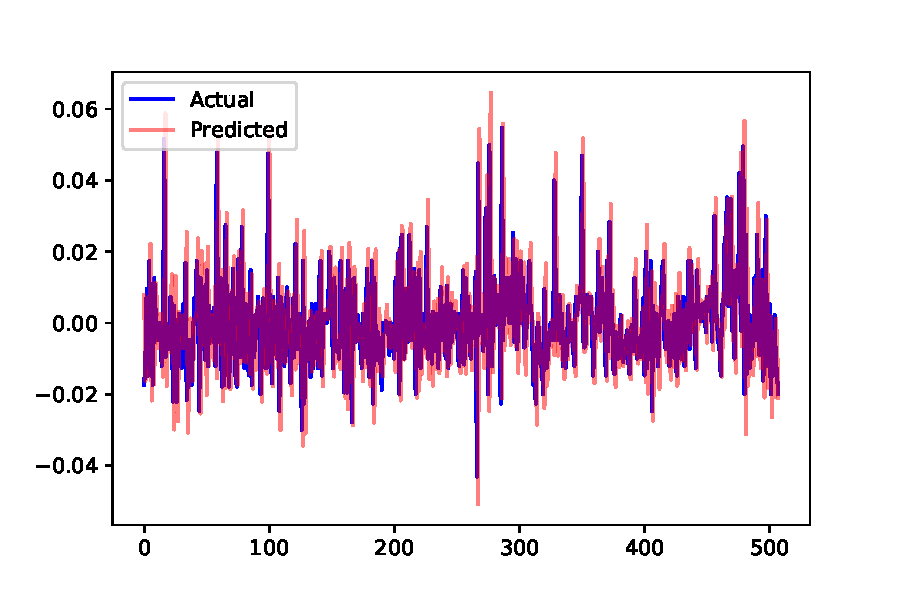
\includegraphics[scale=0.5]{../svm/CS13-ARIMA-differences.pdf}
                \label{fig:ARIMA13}
            \end{figure}
        \end{minipage}
        \begin{minipage}{0.5\textwidth}
            \begin{figure}[H]
                \centering
                \caption{ARIMA 3 to 5 year spread}
                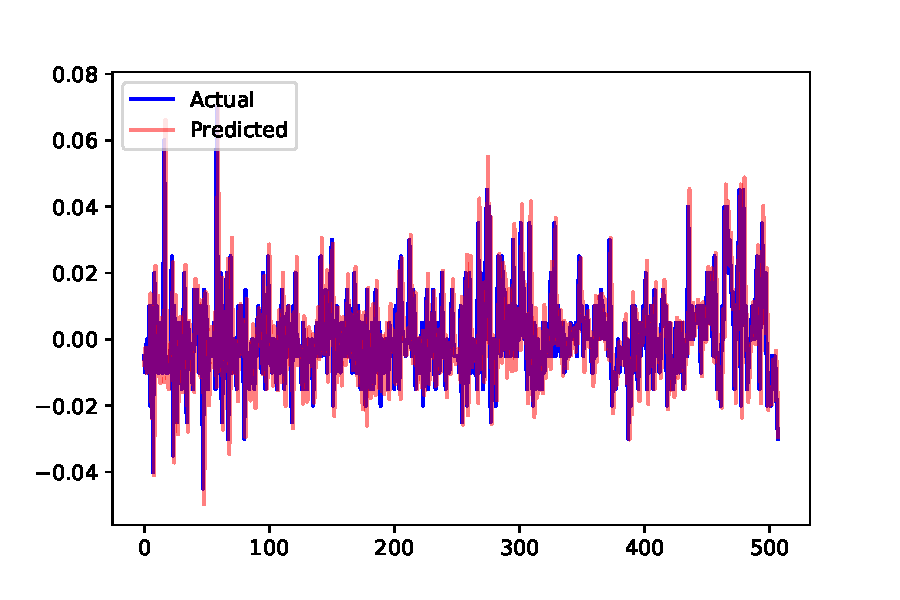
\includegraphics[scale=0.5]{../svm/CS35-ARIMA-differences.pdf}
                \label{fig:ARIMA35}
            \end{figure}
        \end{minipage}

        \begin{minipage}{0.5\textwidth}
            \begin{figure}[H]
                \centering
                \caption{ARIMA 5 to 7 year spread}
                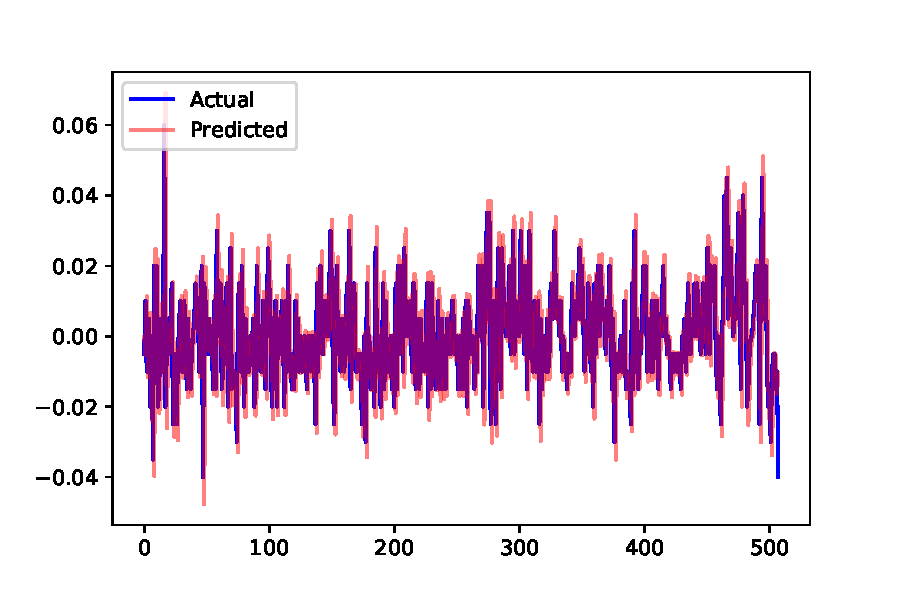
\includegraphics[scale=0.5]{../svm/CS57-ARIMA-differences.pdf}
                \label{fig:ARIMA57}
            \end{figure}
        \end{minipage}
        \begin{minipage}{0.5\textwidth}
            \begin{figure}[H]
                \centering
                \caption{ARIMA 7 to 10 year spread}
                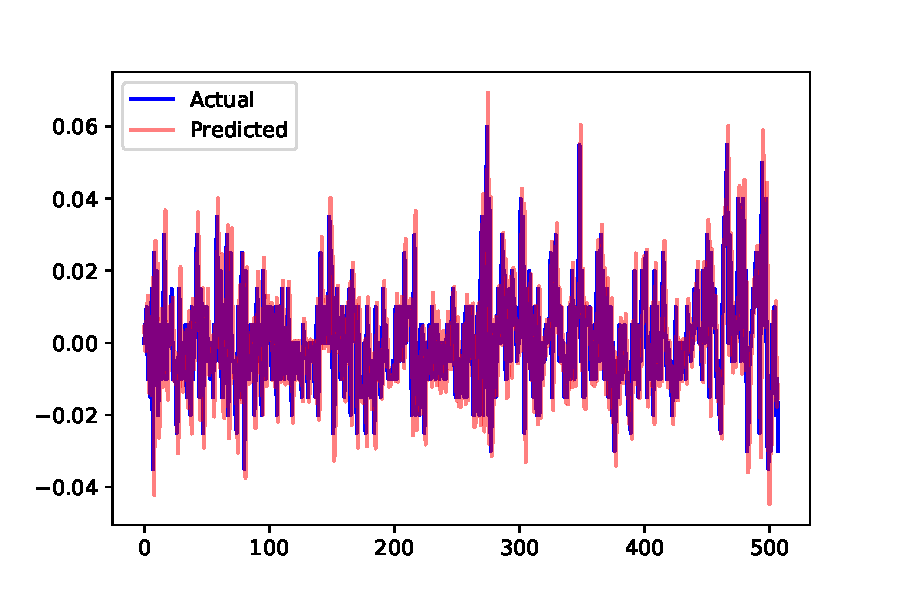
\includegraphics[scale=0.5]{../svm/CS710-ARIMA-differences.pdf}
                \label{fig:ARIMA710}
            \end{figure}
        \end{minipage}

        As we can see, the ARIMA achieves a very low Root Mean Squared Error, but it is very sensitive to high-intensity, low-impact fluctuations in the spread data.
        This is clear evidence of overfitting, and indicative of ARIMA's lack of suitability for predicting the credit spread.

    \subsection{Support Vector Machines}
    We used the \href{https://scikit-learn.org/stable/index.html}{SciKitLearn} module
    \href{https://scikit-learn.org/stable/modules/generated/sklearn.svm.SVR.html}{\texttt{sklearn.svm.SVR}} to implement our Support Vector Machines (SVMs),
    which very conveniently implements a Support Vector Machine for regression instead of classification, which is more useful for our project.
    We were initially going to use a classification SVM to classify future dates into one of either the ``downward trend" or ``upward trend" categories,
    but a regression captures not only this information but also information about the magnitude of a possible downward or upward trend.

    In our SVM, we used the radial basis function (or \texttt{rbf}) kernel and trained the model on the first $5009$ data points,
    using the remaining $500$ data points for validation.

    The data had to be transformed from time-series data to points in $\mathbb{R}^n$ since the SVM is not capable of training directly on time-series data.
    To get around this, the model trained on the difference from one day to the next in the credit spread, labeled by the actual credit spread value for that day.
    The model also does not take into account just one day's spread value to predict the next day's;
    we implemented a $3$-day look-back, so that the spread data for the previous $3$ days was considered for predicting the next day's spread.
    This resulted in having a tall/skinny rectangular, circulant matrix for our training data, instead of a long vector.

    We also implemented $1$-day and $5$-day look-backs, but they did not perform as well as the $3$-day look-back SVM model.
    The SVM's performance on the validation data is summarized by the figures below.

        \begin{minipage}{0.5\textwidth}
            \begin{figure}[H]
                \centering
                \caption{SVM 1 to 3 year spread}
                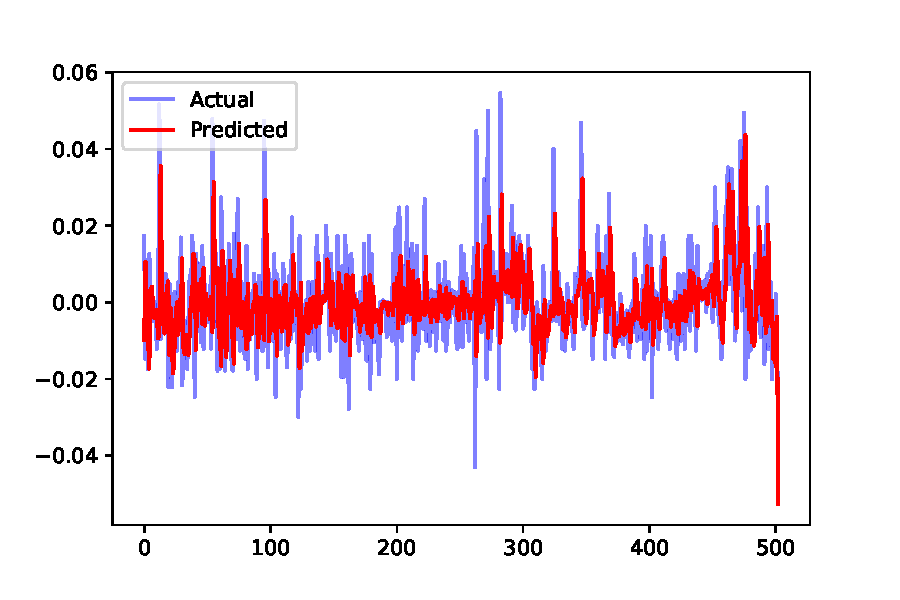
\includegraphics[scale=0.5]{../svm/CS13-3day-lookback-legend.pdf}
                \label{fig:SVM13}
            \end{figure}
        \end{minipage}
        \begin{minipage}{0.5\textwidth}
            \begin{figure}[H]
                \centering
                \caption{SVM 3 to 5 year spread}
                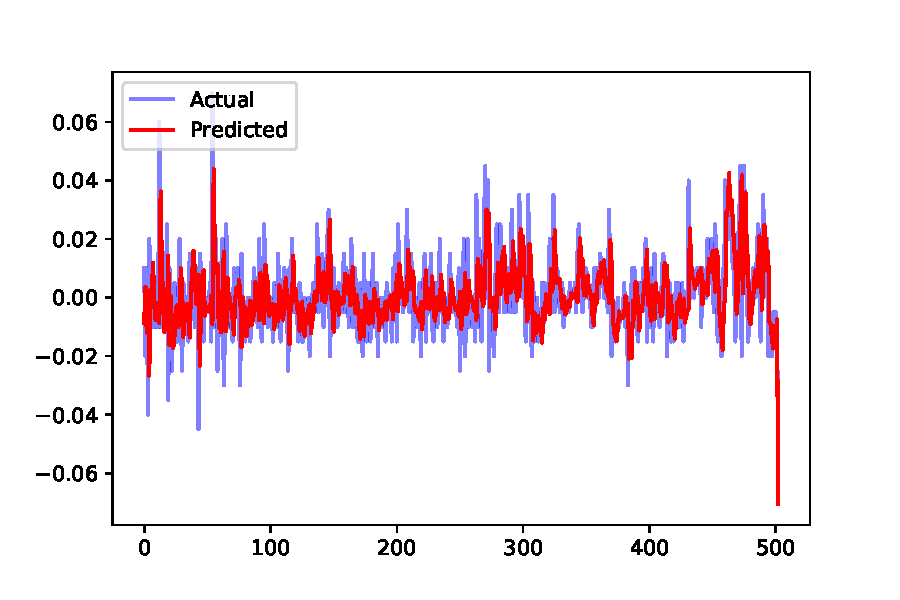
\includegraphics[scale=0.5]{../svm/CS35-3day-lookback-legend.pdf}
                \label{fig:SVM35}
            \end{figure}
        \end{minipage}

        \begin{minipage}{0.5\textwidth}
            \begin{figure}[H]
                \centering
                \caption{SVM 5 to 7 year spread}
                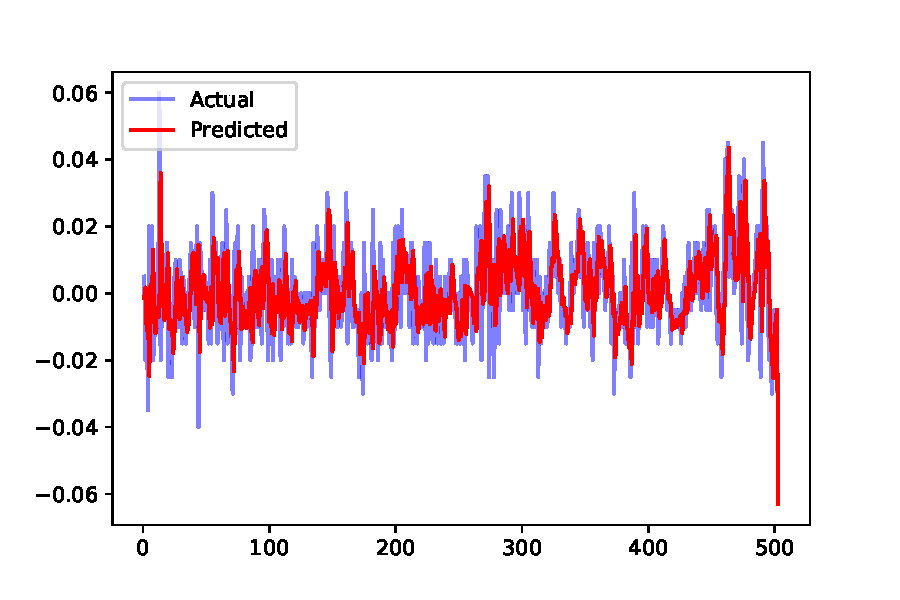
\includegraphics[scale=0.5]{../svm/CS57-3day-lookback-legend.pdf}
                \label{fig:SVM57}
            \end{figure}
        \end{minipage}
        \begin{minipage}{0.5\textwidth}
            \begin{figure}[H]
                \centering
                \caption{SVM 7 to 10 year spread}
                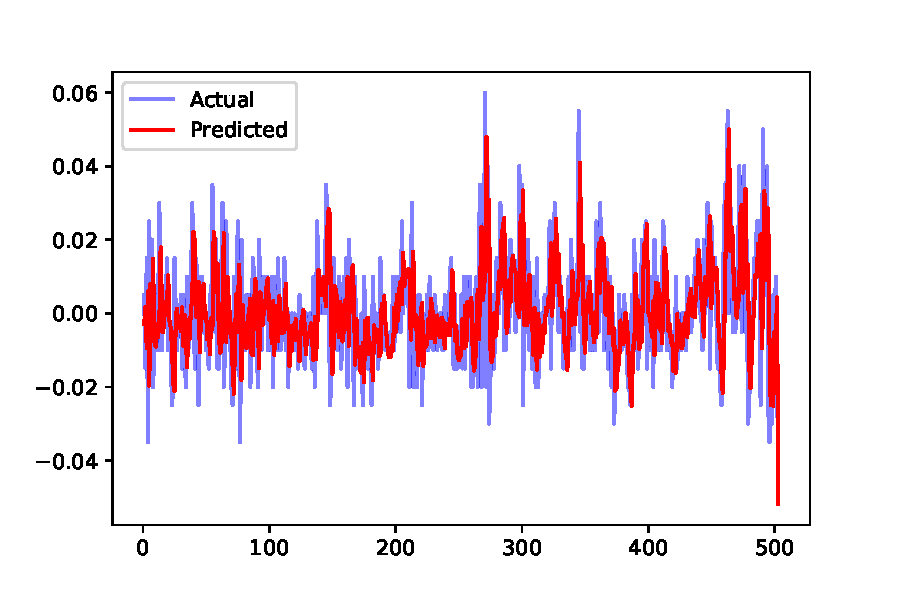
\includegraphics[scale=0.5]{../svm/CS710-3day-lookback-legend.pdf}
                \label{fig:SVM710}
            \end{figure}
        \end{minipage}

        As we can see, the SVM model is predicting a high-magnitude downward trend at the end of the validation set for all of the maturity groups,
        so if we believe the SVM model, we would predict a strong downward shift in the credit spread, which would indicate confidence in the economy, among other things.

        However, the caveat with this model is similar to that of the ARIMA: it is too sensitive to very large but fleeting fluctuations in the credit spread data.
        Therefore, we should not ascribe a high level of confidence to the prediction this model is making.

    \subsection{LSTM Neural Networks}
    Since the SVM seems to perform similarly to the ARIMA model, and both seem to fail to generalize past noise in the data, we attempted to use Neural Networks,
    which are famous for their ability to eschew irrelevant information and learn their own relevant features for the data.
    However, a traditional feed-forward neural network would have trouble learning on time-series data, in a similar manner to the SVM,
    since it is essentially just a function from $\mathbb{R}^n$ to $\mathbb{R}^m$,
    and reducing the input dimension to $n = 1$ would be disastrous for the predictive capabilities of the network.

    We initially had the idea of doing a look-back-based approach, as in the SVM,
    to arrange the data into points in e.g. $\mathbb{R}^3$ to train the network,
    but then we discovered that Long Short-Term Memory (LSTM) neural networks, a kind of recurrent neural network,
    are ideally-suited for making predictions on time-series data.
    As a result, we decided to use the \href{https://www.mathworks.com/help/deeplearning/ug/long-short-term-memory-networks.html}{Regression LSTM Networks} implementation in
    \href{https://www.mathworks.com/products/matlab.html}{MatLab} for our neural network.

    We used a variety of architectures for the neural network, as well as training the network on an assortment of data,
    to compare the relative effectiveness of these choices on the prediction quality.
    First, we used a simple architecture consisting of two sequential LSTM layers, each with $150$ nodes, followed by a fully-connected layer with $150$ nodes,
    which finally produces an output. This architecture was trained the 1 to 3 year maturity credit spread time-series
    in addition to various combinations of exogenous data from Dow Jones, S\&P $500$, NASDAQ, VIX, and the inflation rate.
    For the credit spread time-series, the first $5249$ data points were used for training, and the remaining $260$ were used for validation.
    The performance of these networks on the validation sets, along with graphs of the Root Mean Squared Errors, are presented in the figures below,
    annotated with the exogenous data used to train each model.

    \begin{minipage}{0.5\textwidth}
        \begin{figure}[H]
            \centering
            \caption{DJ, S\&P $500$, NASDAQ, VIX, inflation}
            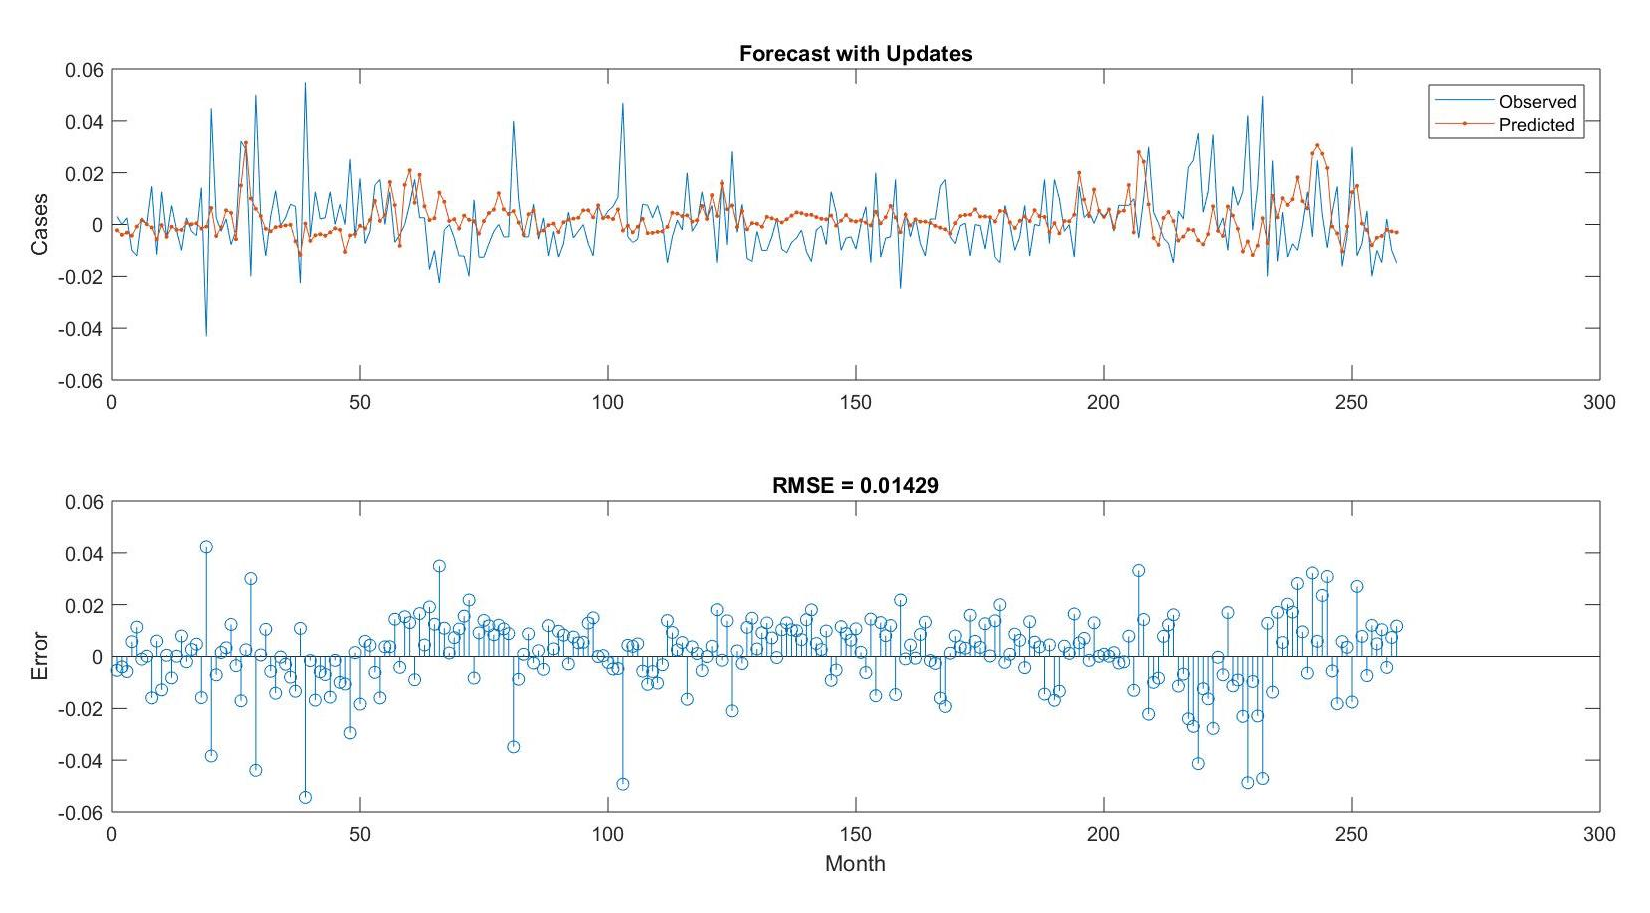
\includegraphics[scale=0.28]{../shreya/lstm1.pdf}
            \label{fig:LSTM-shreya-1}
        \end{figure}
    \end{minipage}
    \begin{minipage}{0.5\textwidth}
        \begin{figure}[H]
            \centering
            \caption{No exogenous data}
            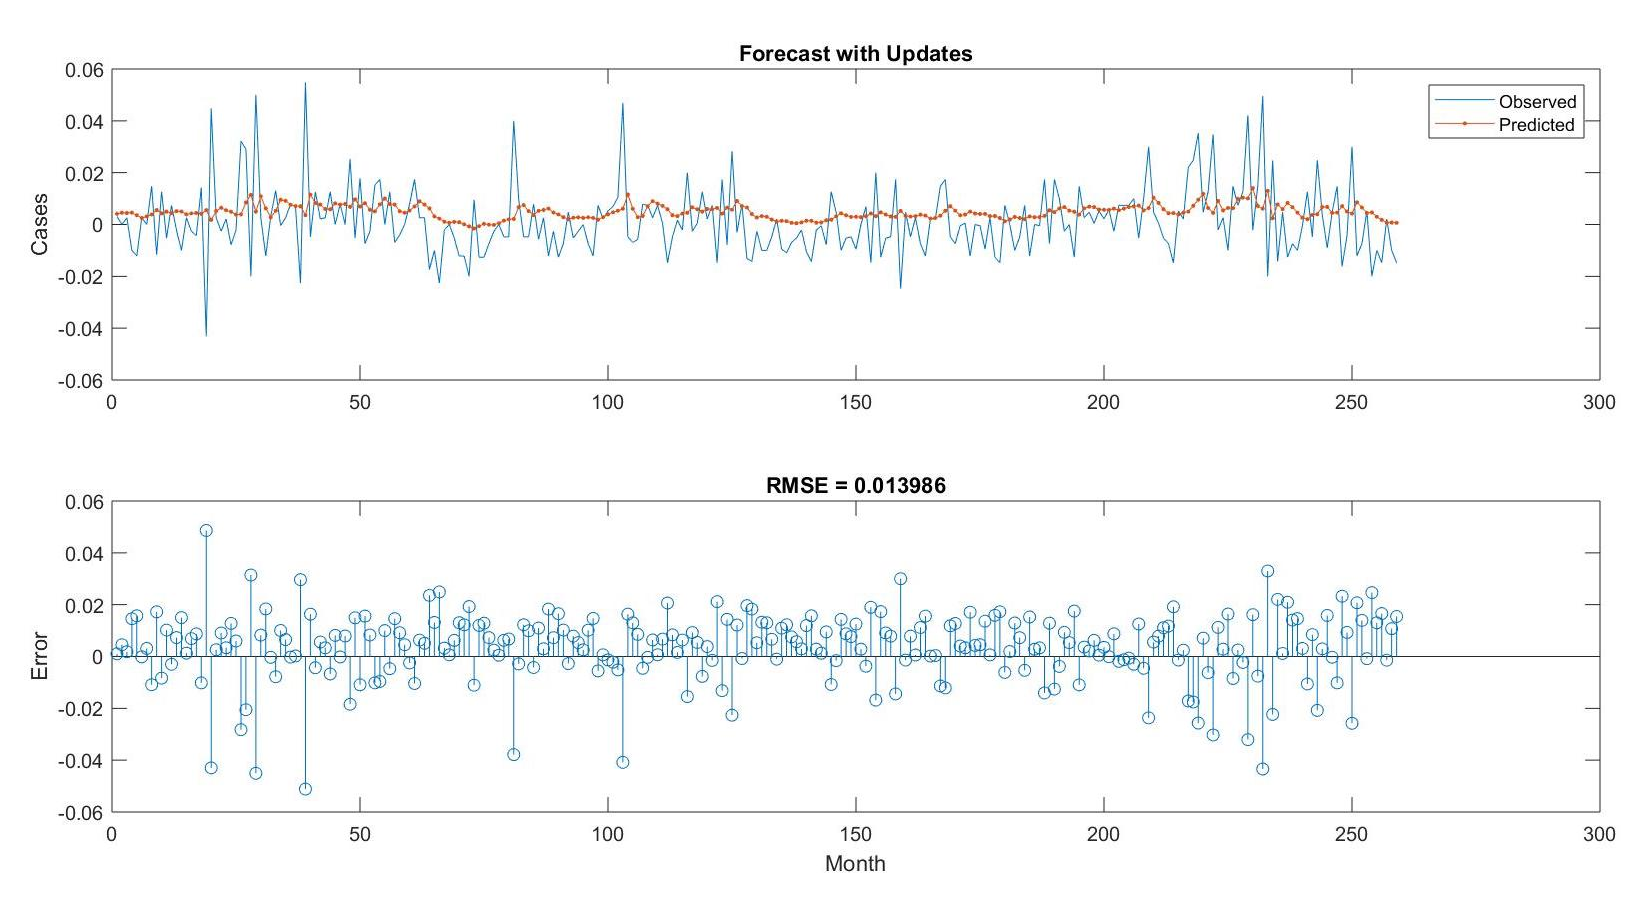
\includegraphics[scale=0.28]{../shreya/lstm4.pdf}
            \label{fig:LSTM-shreya-4}
        \end{figure}
    \end{minipage}

    \begin{minipage}{0.5\textwidth}
        \begin{figure}[H]
            \centering
            \caption{Dow Jones}
            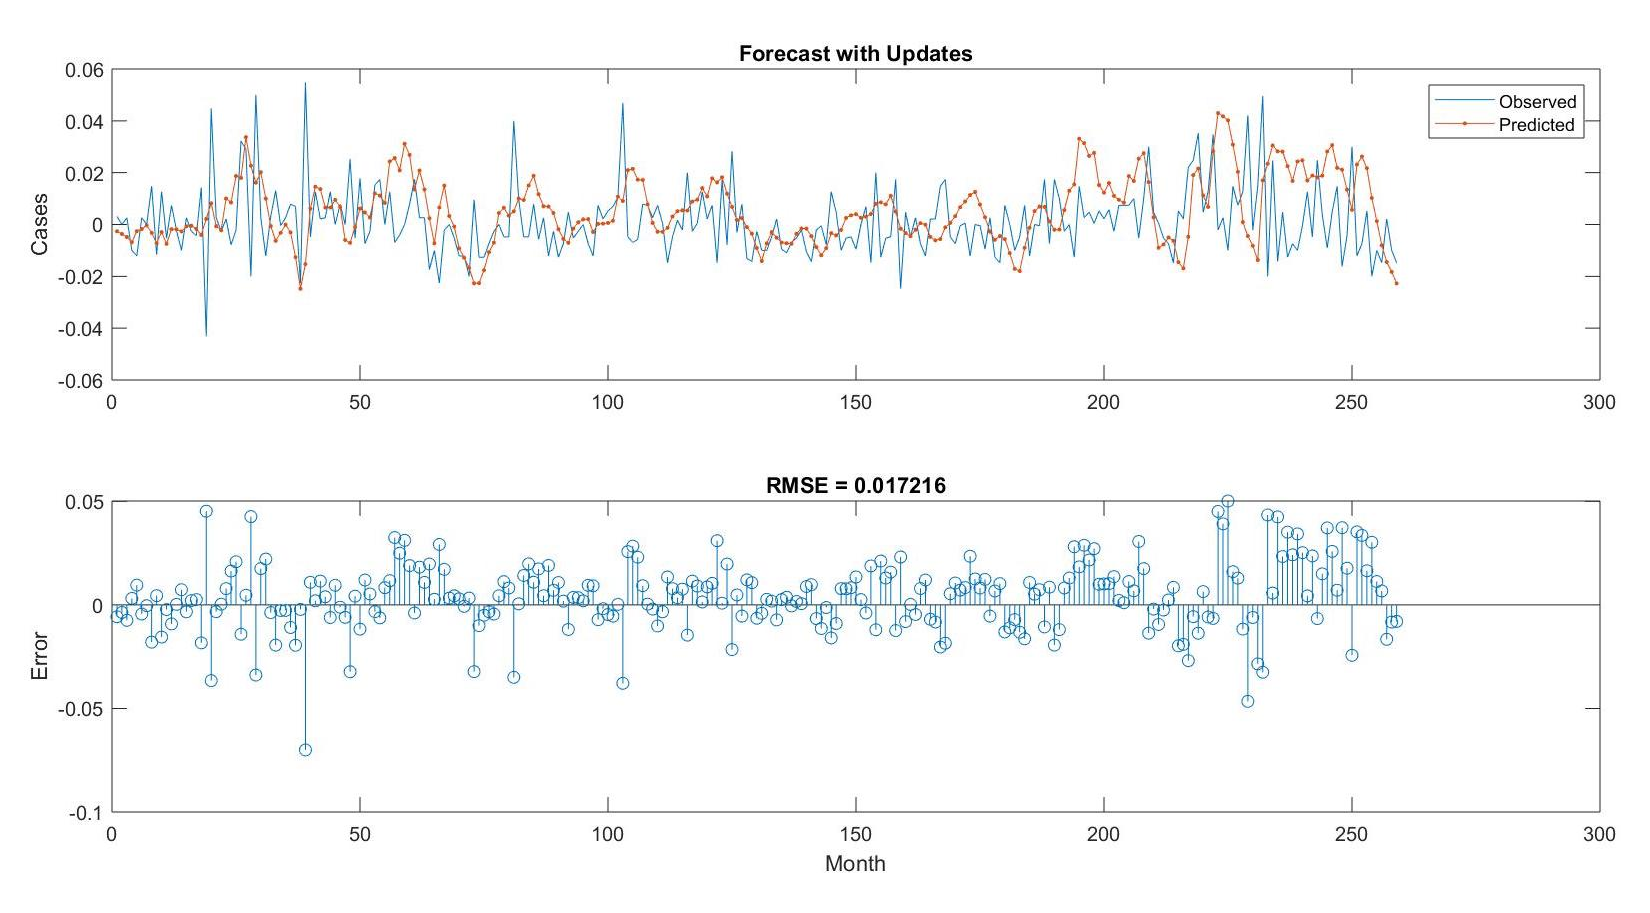
\includegraphics[scale=0.28]{../shreya/lstm2.pdf}
            \label{fig:LSTM-shreya-2}
        \end{figure}
    \end{minipage}
    \begin{minipage}{0.5\textwidth}
        \begin{figure}[H]
            \centering
            \caption{S\&P $500$}
            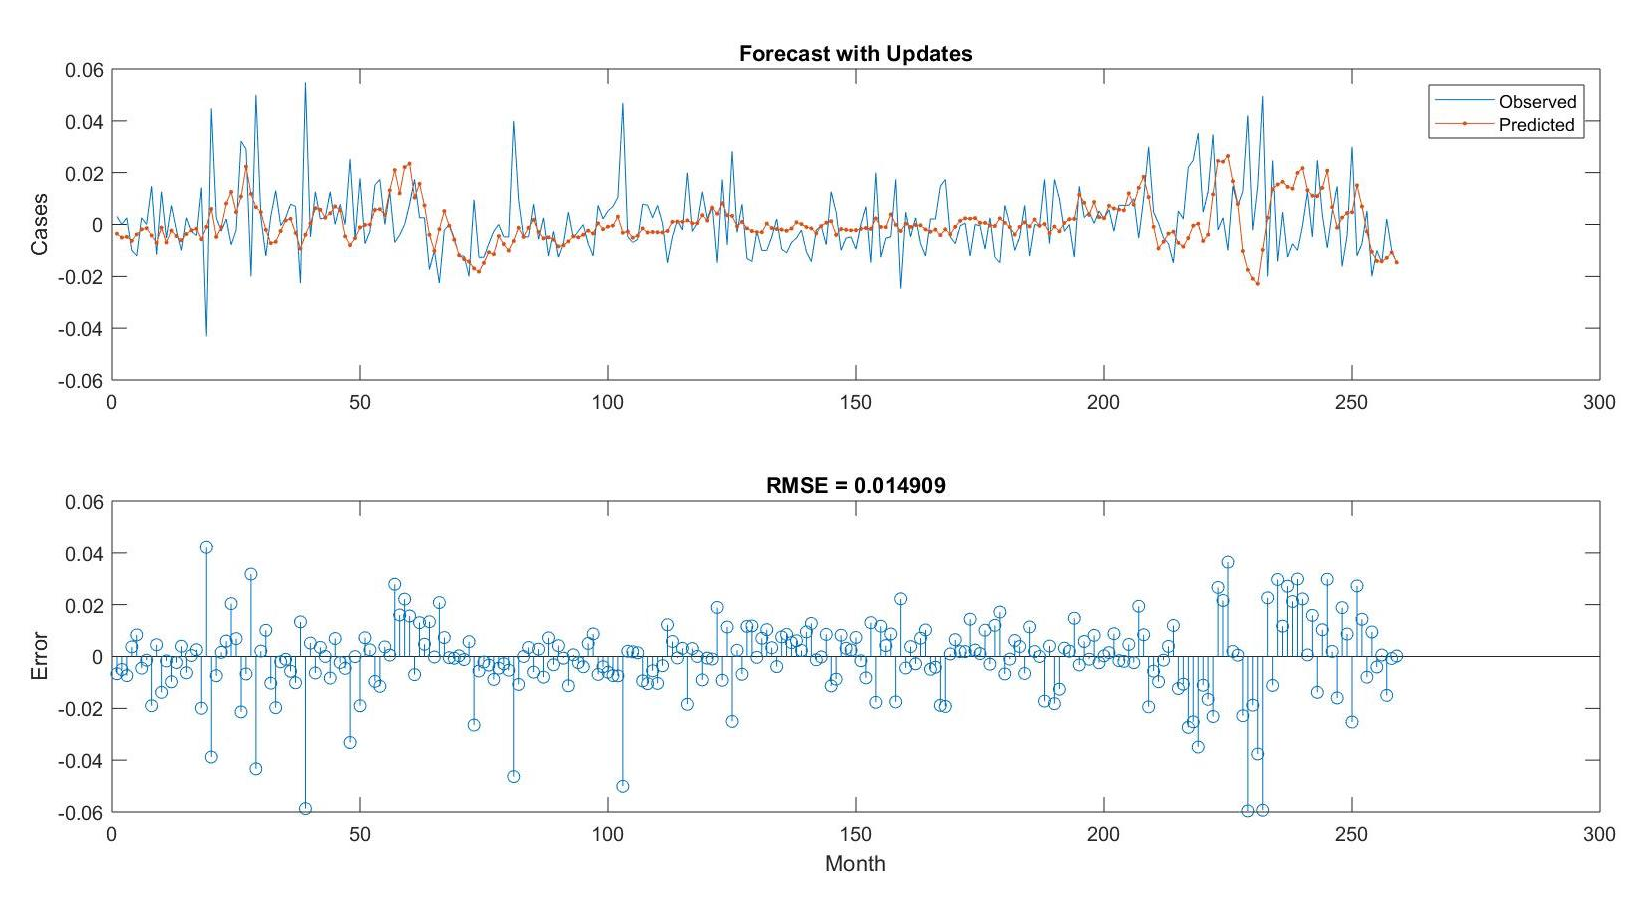
\includegraphics[scale=0.28]{../shreya/lstm5.pdf}
            \label{fig:LSTM-shreya-5}
        \end{figure}
    \end{minipage}

    \begin{minipage}{0.5\textwidth}
        \begin{figure}[H]
            \centering
            \caption{NASDAQ}
            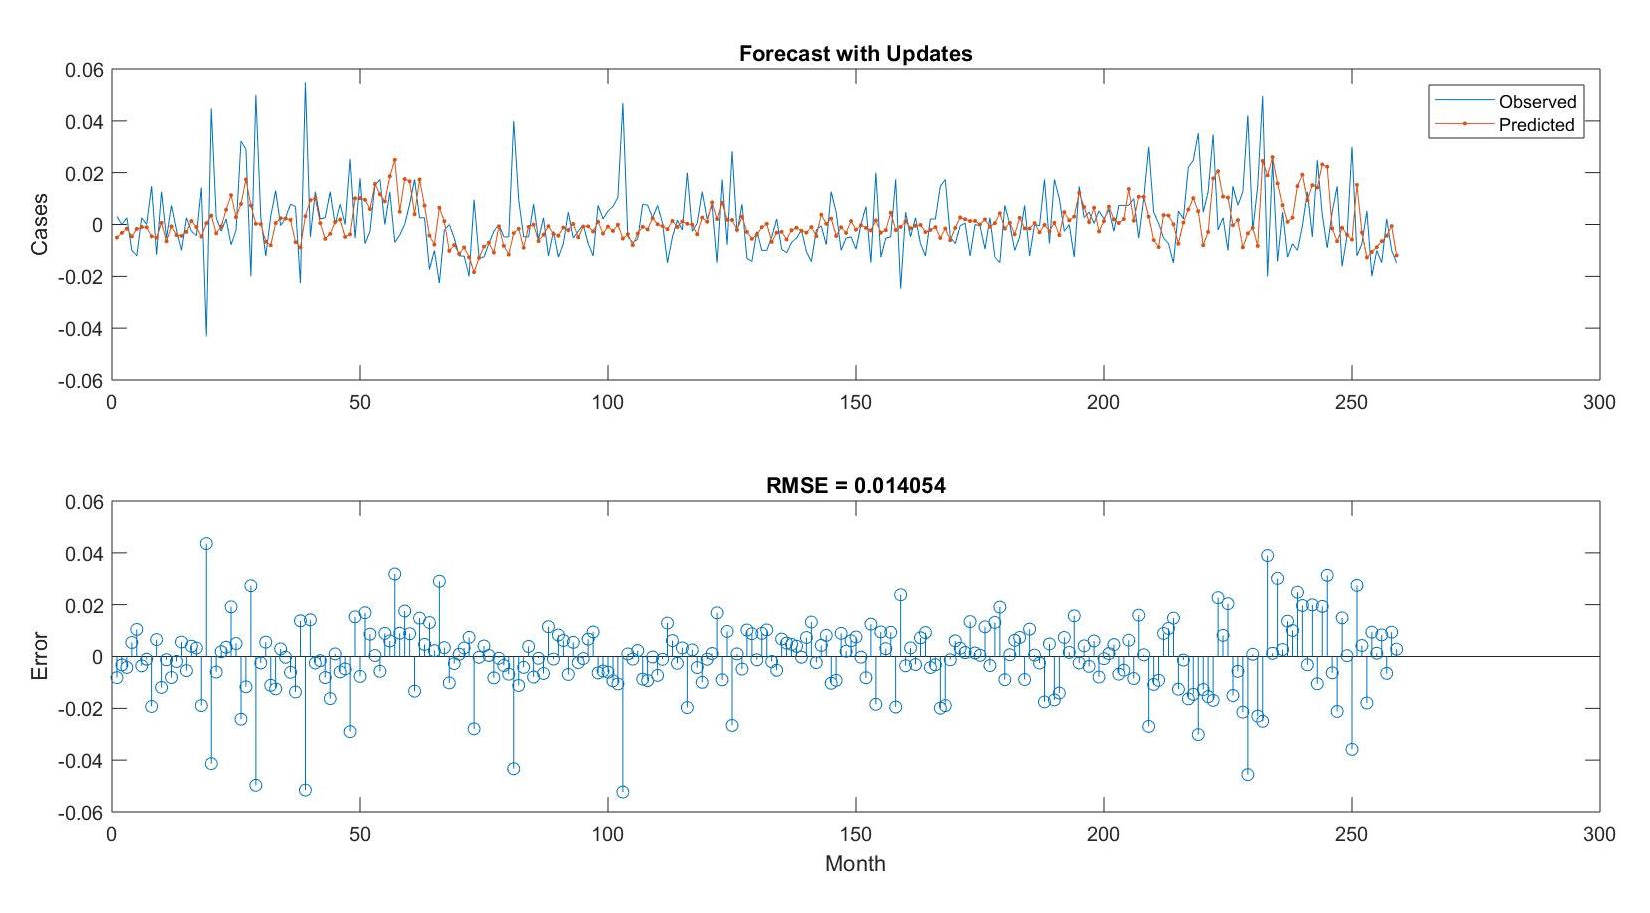
\includegraphics[scale=0.28]{../shreya/lstm3.pdf}
            \label{fig:LSTM-shreya-3}
        \end{figure}
    \end{minipage}
    \begin{minipage}{0.5\textwidth}
        \begin{figure}[H]
            \centering
            \caption{VIX}
            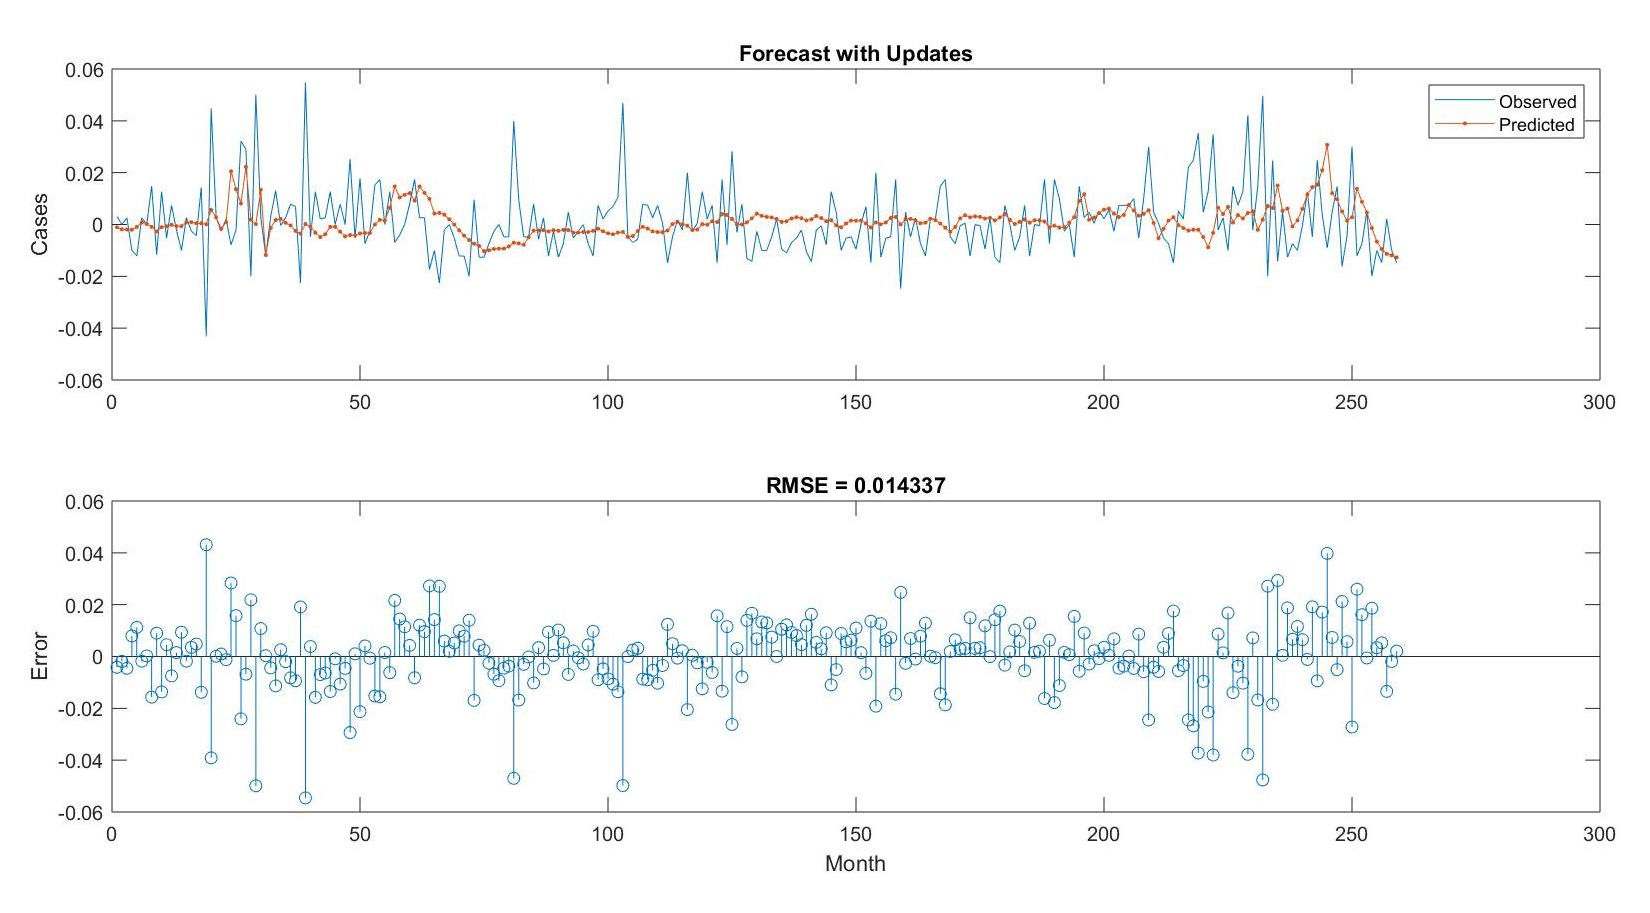
\includegraphics[scale=0.28]{../shreya/lstm6.pdf}
            \label{fig:LSTM-shreya-6}
        \end{figure}
    \end{minipage}

    Next, we tried fixing the data set as the spread data plus S\&P $500$ and VIX and varying the neural network architecture.
    We tried one LSTM layer followed by two fully-connected layers with $100$ nodes each,
    two LSTM layers followed by two fully-connected layers with $100$ nodes each,
    two LSTM layers followed by two fully-connected layers with $50$ nodes each,
    and two LSTM layers followed by two fully-connected layers with $200$ nodes each.
    All of these architectures were trained on the same set of data:
    the credit spread time-series, along with exogenous information from the S\&P $500$ and VIX.
    The first $5259$ points in the credit spread were used for training, while the remaining $250$ were used for validation.
    The performance of the neural networks on the validation sets is presented in the figures below.

    \begin{figure}[H]
        \centering
        \caption{One LSTM layer, two fully-connected layers, $100$ nodes each}
        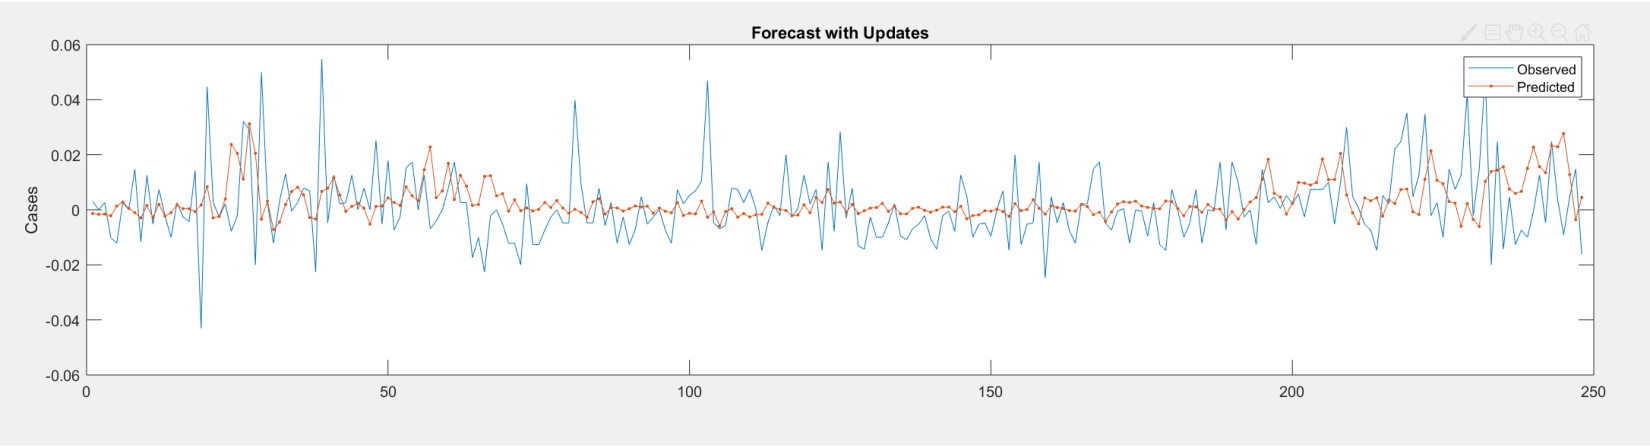
\includegraphics[scale=0.63]{../zezhong/lstm1.pdf}
        \label{fig:LSTM-zezhong-1}
    \end{figure}
    \begin{figure}[H]
        \centering
        \caption{Two LSTM layers, two fully-connected layers, $100$ nodes each}
        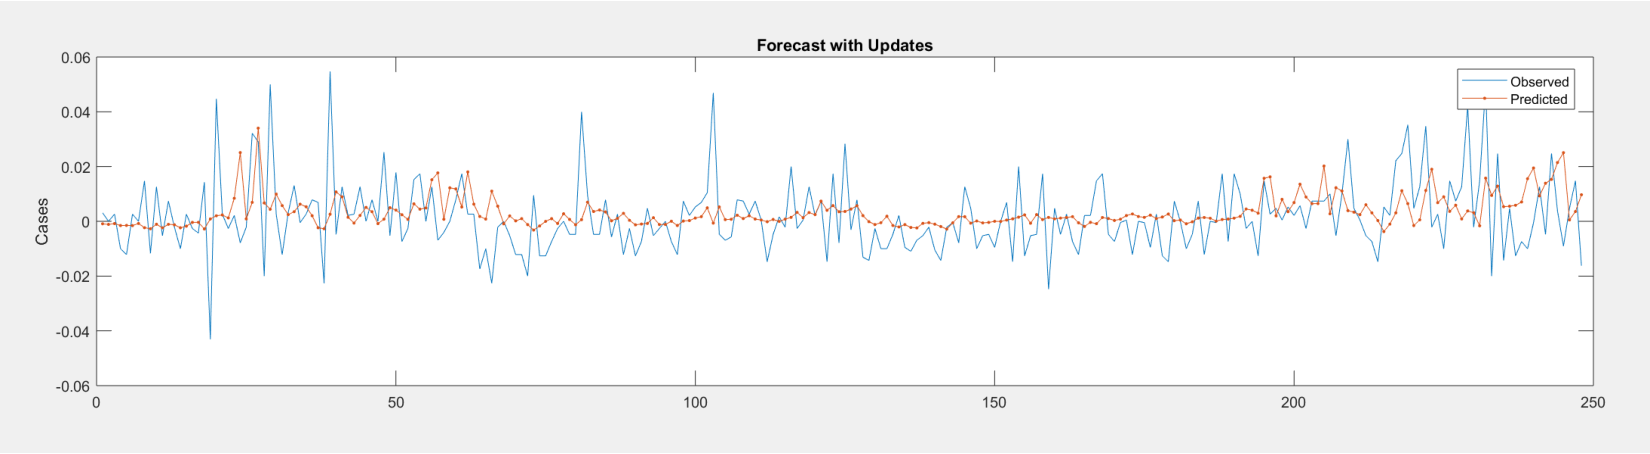
\includegraphics[scale=0.63]{../zezhong/lstm2.pdf}
        \label{fig:LSTM-zezhong-2}
    \end{figure}
    \begin{figure}[H]
        \centering
        \caption{Two LSTM layers, two fully-connected layers, $50$ nodes each}
        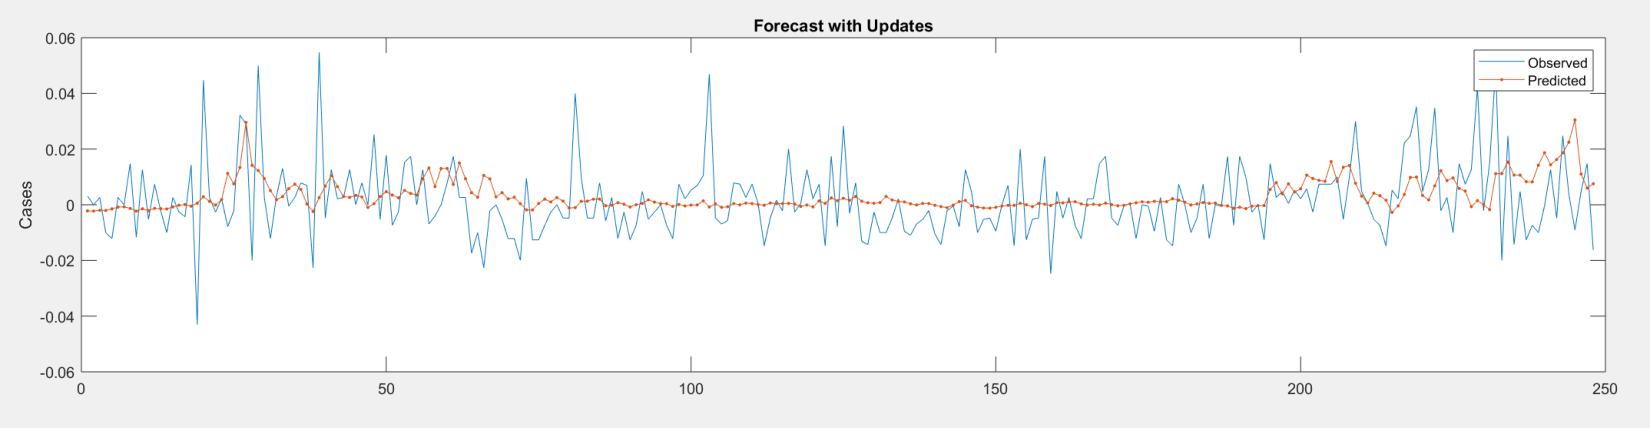
\includegraphics[scale=0.63]{../zezhong/lstm3.pdf}
        \label{fig:LSTM-zezhong-3}
    \end{figure}
    \begin{figure}[H]
        \centering
        \caption{Two LSTM layers, two fully-connected layers, $200$ nodes each}
        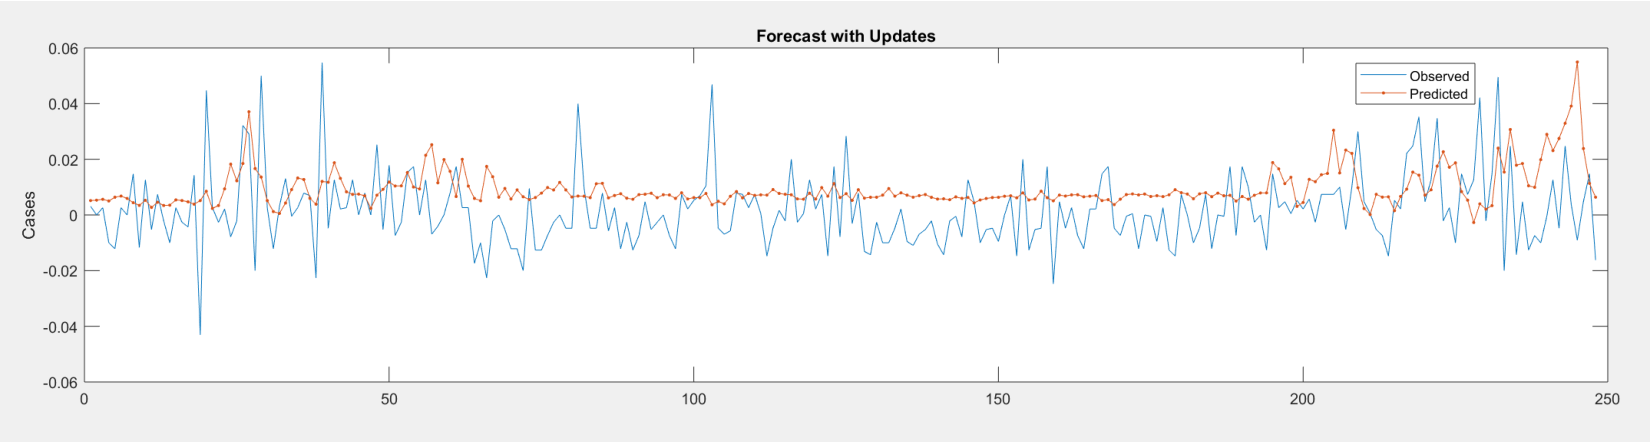
\includegraphics[scale=0.63]{../zezhong/lstm4.pdf}
        \label{fig:LSTM-zezhong-4}
    \end{figure}

    Out of these networks, the one that seems to most accurately capture the rise and fall of the credit spread without overfitting noise is
    \autoref{fig:LSTM-zezhong-2}.
    Note that \autoref{fig:LSTM-zezhong-4} is unreliable, as it has a prolonged period of stability well-above the actual stationary value of the credit spread,
    in addition to predicting a very recent large spike in the spread which is not corroborated by the data.

\section{Summary of Results}
As we saw in the previous sections, the ARIMA benchmark and the SVM both drastically overfit the data,
and therefore their long-term predictions about the credit spread should not be trusted
However, since they seem to follow the data {\it so} closely,
we might reasonably use these models to make short-term predictions about the credit spread with some reasonable level of confidence.
One should be careful, however, not to make predictions on {\it too} short of a term using these models, as there is a slight delay before the models respond
to drastic changes in the credit spread, and thus they will lead to inadequate results if used for e.g. high-frequency trading.
This is to be expected, since, if such a simple method were profitable for short-term trading,
this would represent an arbitrage situation and would violate one of the fundamental assumptions for financial markets
(in addition to undoubtedly having already gained notoriety as sure-fire trading strategy).

Looking now towards the LSTM neural networks, we see that they are much more capable of capturing the essence of the data without overfitting like the ARIMA and SVM models.
After deciding which exogenous data to use, which was the purpose of \autoref{fig:LSTM-shreya-1} through \autoref{fig:LSTM-shreya-6},
we decided that the architecture whose performance is shown in \autoref{fig:LSTM-zezhong-2}
was best able to strike a balance between accuracy of prediction and ability to generalize past the training/validation sets.
This network seems to be predicting a moderate increase in the spread,
which is comfortingly corroborated by the models in \autoref{fig:LSTM-zezhong-1} and \autoref{fig:LSTM-zezhong-3} as well.
The only one of these networks that disagrees is \autoref{fig:LSTM-zezhong-4},
which seems to think there was a large spike in the credit spread very recently which we are just now recovering from (which is not warranted from the data).

Therefore, we should reasonably conclude that the credit spread is due for a marginal increase.

\end{document}
